\chapter{Representação Gráfica de Dados}
\section{Desenvolvimento Histórico}

As origens da visualização ou representação estão nos diagramas geométricos, nas tabelas de posição das estrelas e nos mapas. No século XVI, com a expansão marítima da Europa, novas técnicas e instrumentos foram desenvolvidos e, com eles, novos, e mais precisas, forma de apresentação visual do conhcecimento. Até meados do século 17, ocorreram os primeiros mapas e diagramas.\vskip0.3cm


Durante meados de 1600 a 1699, período este chamado de Medições e Teorias, os maiores problemas do século se referiam a medição física do tempo, distância e espaço para astronomia, nevegação e expansão terrotorial. Avannçam as estimativas, as probabilidades, a demografia e todo o campo de estatística. No fim do século os elementos para iniciar um pensamento visual então prontos. \vskip0.3cm


\par Entre 1700 a 1799, conhecido como das novas fórmulas gráficas, cartógrafos começam a mostrar mais do que a posição geográfica. Até o fim do século aparecem tentativas de mapear informações de geologia, economia, demografia e saúde. A medida que o volume de dados avança, novas fórmulas de visualização aparecem. Inovações tecnológicas como a cor, litografia e imprenssa abrem novos caminhos. Em 1786, Willian Playfair produziu os primeiros gráficos de linhas, barras e setores.



\vspace{-1.5cm}
\begin{figure}
    \centering
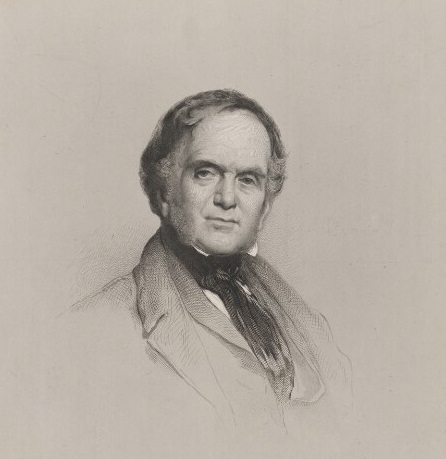
\includegraphics[scale=0.35]{figures/william_playfair.jpeg}
    \caption{William Playfair (1759-1823)}
    \label{fig:my_label4}
\end{figure}







A primeira metade do século XIX, conhecido com Início da Infografia Moderana (1800 à 1849), foi responsável por uma explosão no crescimento de gráficos estatísticos e de mapeamento temático, graças as inovações obtidas no século anterior. Todas as formas de gráficos estatísticos conhecidas hoje foram desenvolvidas nesta época, na cartografia, mapas simples foram transformados em atlas complexos baseados em grande variedade de dados.  
\vskip0.3cm

\inic Entre os anos de 1850 à 1900, conhecido como Era de Ouro da Estatística, onde as condições para um rápido crescimento das visualizações estavam estabelecidos. Escritórios de Análises se espalhavam pela Europa com o aumento da importância das informações numéricas para planejamento social, industria, comércio e transporte. A teoria estatística iniciada por GAUSS e LAPLACE deu os meios para fazer sentido a um grande número de dados.  
\vskip0.3cm 


\inic Compreendido entre 1900 à 1949, chamado de Período Negro do Gráficos de Estatística, aconteceram poucas inovações gráficas e o entusiasmo vivido no século passado foi suplantado pelo crescimento da quantificação e modelos formais. Durante esse período, no entanto, tudo que foi alcançado consegue se popularizar, seja no governo, no comércio e nas ciências. A visualização gráfica é consagrada para explicar novas descobertas e teorias.
\vskip0.3cm 


\inic De 1975 até hoje, o computador é considerado como nova fronteira. As inovações ocorridas nesta época foram muitas e em diversas áreas: o desenvolvimento de softwares e sistemas de computador,
altamente interativos e de fácil manipulação, foram a alavanca para tudo.\vskip0.3cm  

%Os novos paradigmas de manipulação de dados, a
%invenção de técnicas gráficas e os métodos de vizualização multidimensional deixaram suas marcas também.\vskip0.3cm  

\inic Com o surgimento da multimídia e da internet nos anos
1990 foram multiplicadas as formas de representar informação de modo dinâmico,
explorando animações, gráficos interativos e mapas com escala variável.






\newpage
\section{Autores Importantes na Representação Gráfica}

\begin{itemize}


\item O médico anestesista Britânico John Snow considerado o pai da epidemiologia moderna, em 1854, descobre a fonte transmissora de cólera e com um mapa registrou as coordenadas das ocorrências dos óbitos (SNOW, 1854a);

%\vspace{-1.5cm}
%\begin{figure}
%   \centering
%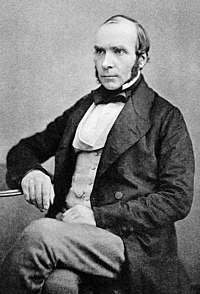
\includegraphics[scale=0.6]{figures/John_Snow.jpeg}
%    \caption{John Snow (1759-1823)}
%    \label{fig:my_label4}
%\end{figure}

\item Em 1858, Florence Nightingale, enfermeira britânica produziu o coxcomb diagrams que mostrou as baixas do exército britânico na Guerra da Criméia;

%\vspace{-10cm}
% \begin{figure}
 %   \centering
%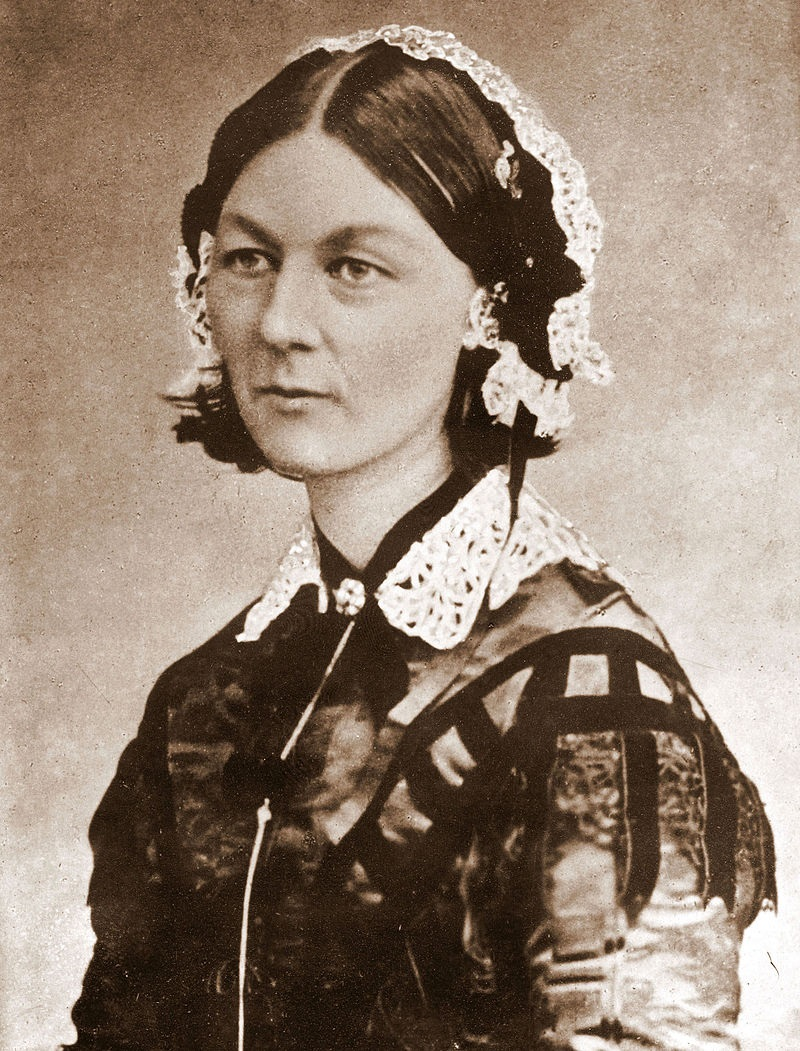
\includegraphics[scale=0.4]{figures/Florence_Nightingale.jpeg}
%    \caption{Florence Nightingale(1759-1823)}
%    \label{fig:my_labe34}
%\end{figure}
  

\item Durante o ano de 1869, Charles Joseph Minard, engenheiro civil francês retratou a dizimação do exército de Napoleão durante sua condenada campanha contra a Rússia. Desmonstrando como níveis mais complexos de narratividades podem ser alcançados com uma única visualização estática (MINARD, 1869);
\item No ano de 1914, Willard Brinton engenheiro americano publicou o primeiro livro de visualização para negócios;
\item Em 1952, Mary Eleanor Spear publicou seu livro contendo boas práticas em construção de gráficos baseadas em décadas de serviço no governo Americano;
\item Em 1967, Jacques Bertin, cartógrafo francês publicou o primeiro livro sobre teoria da visualização (Sémiologie graphique: Les diagrames, les
réseaux, les cartes), criava um sistema complexo de representação visual, com destaque para a cartografia. A semiologia gráfica era uma proposta arrojada para colocar problemas e apresentar dados de grande complexidade, longe de ser apenas ilustrativa (BERTIN, 1967); O livro era uma síntese de duas décadas de trabalho cotidiano na preparação de mapas para ilustrar livros de história e ciências sociais (GIL e BARLETA, 2015);
\item Em meados de 1970, John Tukey matemático americano foi pioneiro no uso de computadores para visualização e popularizou o conceito de visualização exploratória e confirmatória (TUKEY, 1997);
\item Em 1983, Edward Rolf Tufte publicou em seu livro formas de combinar rigor estatístico com clareza e princípios de design gráfico, ou seja, a excelência em gráficos estatísticos consiste em idéias complexas comunicadas com clareza, precisão e eficiência (TUFTE, 1983);
\item Em 1986, Jock Mackinlay publicou sua Tese de PhD que levou o trabalho de Jacques Bertin para era digital;
\item Em 1999, Leland Wilkinson estabeleu uma grámatica concisa para descrever os componentes de um gráfico.
\end{itemize}



\section{Porque usar Gráficos}

As estatísticas geralmente podem ser melhor compreendidas quando são apresentadas em um gráfico do que em uma tabela. Um gráfico é uma representação visual de dados estatísticos, em que os dados são representados por símbolos como barras ou linhas.
\vskip0.3cm  

É uma ferramenta visual muito eficaz, pois exibe os dados de forma rápida e fácil, facilita a comparação e pode revelar tendências e relacionamentos dentro dos dados.\vskip0.3cm  

Um gráfico geralmente assume a forma de uma figura uni ou bidimensional, como um gráfico de barras ou um gráfico de linhas. Embora existam gráficos tridimensionais disponíveis, eles geralmente são considerados complexos demais para serem facilmente compreendidos.\vskip0.3cm  

Os gráficos podem ser usados para ilustrar padrões em uma grande quantidade de dados ou para comunicar uma descoberta ou mensagem chave. Você deve considerar o uso de gráficos se quiser mostrar:

\begin{itemize}
    \item \textbf{Comparação}: Quantos? Qual item é maior ou menor?
    \item \textbf{Mudanças ao Longo do Tempo:} Como uma variável evolui?
    \item \textbf{Distribuição de frequência}: Como os itens são distribuídos? Quais são as diferenças?
    \item \textbf{Correlação}: Duas variáveis estão ligadas?
    \item \textbf{Participação relativa de um todo}: como um item se compara ao total
\end{itemize}

\newpage
\section{Quando Pode Não ser Apropriado usar Gráficos}

Um gráfico nem sempre é a ferramenta mais adequada para apresentar informações estatísticas. \vskip0.3cm

Às vezes, um texto e/ou tabela de dados pode fornecer uma explicação melhor para o seu público e economizar tempo e esforço consideráveis.\vskip0.3cm

Você deve reconsiderar o uso de gráficos quando seus dados: 

\begin{itemize}
\item Estiverem muito dispersos; 
\item Têm poucos valores; 
\item Ter muitos valores; 
\item Mostram pouca ou nenhuma variação
\end{itemize}

%ROBINSON, Arthur. The look of maps: An examination of cartographic design. Wisconsin: University of Wisconsin Press, 1952


%SNOW, John. “The Principles on Which the Treatment of Cholera Should Be Based”. Medical Times and Gazette, n.8, 1854a,p.180-2.

%MINARD, Charles Joseph. Carte figurative des pertes successives en %hommes de l’Armée française dans la
%campagne de Russie 1812–1813. Paris: Regnier et Dourdet, 1869.

%TUFTE, Edward. The visual display of quantitative information. 2a edição. Cheshire, Conn.: Graphics
%Press, 2001; TUFTE, Edward. Envisioning information. Cheshire, Conn.: Graphics Press, 1995;

%TUKEY, John W. Exploratory data analysis. Reading, Mass.: Addison-Wesley Pub. Co., 1997

%1983: The Visual Display of Quantitative Information (pictures of numbers). ISBN 0-9613921-0-X

%\newpage
\section{Conceitos Básicos de Representação Gráfica}

\inic Com palavras, números ou desenhos podem-se mostrar às pessoas interessadas o resultado da pesquisa, antes mesmo de aplicarem-se sobre os dados as operações matemáticas, que permitirão a interpretação final por parte da equipe encarregada do levantamento estatístico.\vskip0.3cm

A exposição por palavras é dita descritiva, a numérica é também conhecida como tabular e, finalmente, os desenhos constituem a exposição gráfica. Um relatório final reúne, quase sempre, as três modalidades de exposição, apresentando: gráficos, para ilustrar ou acentuar determinados itens: tabelas, para resumir a massa de dados observados no período de atividades; e palavras, para orientar a leitura, comentar as tabelas analisar os gráficos e concluir o relatório.\vskip0.3cm

Em muitas situações a apresentação gráfica é preferível a apresentação tabular. Os gráficos têm um impacto visual e uma facilidade de interpretação que o tornam muitas vezes mais úteis que as tabelas.\vskip0.3cm

A representação gráfica das séries estatísticas tem por finalidade representar os resultados obtidos, permitindo que se chegue a conclusões sobre a evolução do fenômeno ou sobre como se relacionam os valores da série. A escolha do gráfico mais apropriado ficará a critério do analista.\vskip0.3cm

As representações dos dados em sua forma gráfica constituem
importantes instrumentos de comunicação rápida, clara e efetiva,
poupando, sobretudo, tempo e esforço na visualização de dados
resumidos, permitindo fixar uma imagem duradoura, daí o largo uso
dessas representações em trabalhos científicos atualmente. (Ayres,
2003).\vskip0.3cm

A estatística gráfica são representações visuais dos dados
estatatísticos que devem corresponder, mas nunca substituir as
tabelas estatísticas.


%\newpage
\section{Classificação Didática dos Gráficos}

\subsection{Quanto a Forma}

Há três tipos de gráficos, classificados quanto ao critério da forma:

\begin{enumerate}
  \item \textbf{Diagramas}: os diagramas são gráficos geométricos dispostos em duas dimensões. Os diagramas são os gráficos mais usados na representação de séries estatísticas e se  apresentam através de uma grande variedade de tipos.
\item \textbf{Cartogramas}: os cartogramas são ilustrações relativas a cartas geográficas, largamente difundidas em Geografia, História e Demografia.
\item \textbf{Estereogramas}: os estereogramas representam volumes e são apresentados em três dimensões. Muitas vezes são confeccionados em cartolinas ou madeira quando não desenhados em perspectiva.
\end{enumerate}

\subsection{Quanto ao Objetivo e Uso}

É possível distinguir, de certo modo arbitrariamente, dois objetivos que justificariam o emprego de gráficos. Os gráficos são usados para apresentar visualmente dados numéricos, proporcionando maior facilidade e rapidez de compreensão dos mesmos, ou, então, para apresentar conclusões ou resultados de uma análise. Há portanto, dois tipos de gráficos, conforme o objetivo ou uso a que se destinam: gráficos de informações e gráficos de análise.

\newpage
\subsubsection{Gráfico de Informação}

\inic São gráficos destinados principalmente ao público em geral, objetivando proporcionar uma visualização rápida e clara da intensidade das modalidades e dos valores relativos ao fenômeno observado. São gráficos tipicamente expositivos, devendo, por conseguinte, ser o mais o completo possível, dispensando comentários explicativos adicionais. Nos gráficos de informação não se deve prescindir dos títulos. Já as legendas podem ser omitidas, desde que as informações desejadas  estejam presentes, possibilitando a completa interpretação do gráfico.

\subsubsection{Gráfico de Análise}

\inic Os gráficos de análise prestam-se melhor ao trabalho estatístico, fornecendo elementos úteis à fase de análise dos dados, sem deixar se ser também informativos. Quando se usam gráficos para apresentar os resultados de uma análise, esses freqüentemente vêm acompanhados de uma tabela. Inclui-se, muitas vezes, um texto dissertativo, chamando a atenção do leitor para os pontos principais revelados pelo gráfico ou pela tabela. Muitos relatórios administrativos, econômicos ou de qualquer outra natureza combinam as três formas de apresentação de dados. Isto porque, na prática, poucas pessoas têm habilidade com números, e as que têm dificuldades consultarão, via de regra, apenas o gráfico. Por outro lado, a maior parte das pessoas nunca examinará as tabelas estatísticas, preferindo analisar os gráficos e eventualmente procurar no texto a informação adicional necessária.\vskip0.3cm




\section{Elementos  Básicos na Construção de Gráficos}

\inic Assim como tabelas, os gráficos devem ser referenciados no texto. Se eles ocorrem em um trabalho, é porque possuem alguma importância, fornecem alguma informação. Portanto, eles precisam ter alguma explicação ou comentário a respeito deles no corpo do trabalho.\vskip0.3cm 

\inic A representação gráfica deve conter determinados elementos que são essenciais para a sua compreensão, sendo esses elementos:



\newpage
\section{Elementos Básicos}

\begin{itemize}
\item \textbf{Número}: utilizado para identificar o gráfico no
texto, sendo sempre precedido da palavra GRÁFICO com o seu número.
Por exemplo: GRÁFICO 1, GRÁFICO 2 etc, ou de acordo com a
numeração do capítulo, GRÁFICO 1.1, GRÁFICO 1.2, e assim por
diante. \item \textbf{Título}: deve conter designação do fenômeno
observado (O QUE?) e o local (ONDE?) e data de ocorrência do mesmo
(QUANDO?) e (COMO?), ficando abaixo do gráfico. O título deve
preferencialmente ser escrito após o número do gráfico, devendo
ser separado por espaço, hífen e espaço em letras maiúsculas
seguindo o padrão do texto. O título deve estar presente em qualquer tipo de representação gráfica a ser escrito com vista a orientar o leitor na sua interpretação. Simultaneamente, deve ser conciso, relevante e claro, ou seja, conter apenas informação essencial para uma interpretação correta do gráfico. 
\item \textbf{Fonte}: indicação do
órgão ou entidade responsável pelo fornecimento dos dados usados
na elaboração do gráfico. Utilizar letras maiúsculas para escrever
FONTE, devendo ser seguida de dois pontos, espaço e o nome da
fonte utilizada. Quando os dados foram obtidos pelo próprio autor,
por exemplo, em uma pesquisa e campo, a fonte pode ser escrita
como: FONTE: o autor. \item \textbf{Nota}: quando necessária, é
utilizada para a apresentação de informações de natureza geral,
esclarecendo o conteúdo ou metodologia utilizada. A nota vem em
seguida à fonte. A palavra NOTA deve ser escrita em letras
maiúsculas, devendo ser seguida de dois pontos, espaço e a
explicação da nota. \item \textbf{Nota Específica}: quando
necessária, é utilizada para esclarecer dados sobre um item ou uma
parte específica do gráfico; empregam-se chamada, indicadas no
gráfico, geralmente no titulo ou na legenda. A nota específica
deve ser chamada por algarismos arábicos entre parênteses.
\item \textbf{Legenda}: a legenda é constituída por símbolos e respectivas designinações. O procedimento dos sinbolos (cor ou outros) deve ser realizado de modo a que não haja lugar para qualquer confusão visual entre eles e, consequentemente, para que exista uma ligação clara entre os simbolos e a componente representada. As desiginações, por seu lado, devem ser claras e concisas, deixando para notas adjascentes eventuais esclarecimentos. Os símbolos devem aparecer na mesma ordem que as respectivas componentes: horizontalmente quando estão lado a lado e verticalmente quando estão umas sobre as outras (WALLGREN, 1996). Uma boa legenda deve fazer mais do que simplesmente etiquetar as componentes do gráfico. Deve dizer-nos o que é importante e qual é o objetivo do gráfico:   
informar o leitor e obrigar quem faz o gráfico a estruturar a informação (CLEVELANDO e MCGILL, 1984a).\vskip0.3cm

\item \textbf{Escalas}: Em um gráfico, as informações que possuem uma escala devem ser apresentadas com clareza. Os números da escala devem estar na posição horizontal e na região
externa dos eixos. A unidade de medida deve aparecer no final de cada linha do gráfico. Caso não seja possível apresentar a escala por completo, pode-se fazer um corte no eixo correspondente para informar que a escala não está completa.

\item \textbf{Linhas Auxiliares}: um dos elementos gráficos visualmente mais monótonos são as linhas auxiliares. devem, por isso ser suprimidas ou abafadas de tal forma que sua presença se torne implícita. Ainda que possam auxiliar a leitura dos dados, a maioria das linhas auxiliares escuras tem um grande peso visual, encobrindo muitas vezes, o mais importante do gráfico: a informação. Quando foram realmente necessárias deve-se optar por usar uma cor neutra e, no caso particular de um fundo branco, a cor cinzenta. Em certos caos em particular nas séries temporais, pode ser considerado importante incluir linhas auxiliares verticais como auxilio a leitura de valores por forma a complementar a leitura evolutiva da série com a leitura de valores em particular. Na maioria dos gráficos de séries temporais, os dados mais recentes estão situados à direita e longe das identificações do eixo dos valores, normalmente localizados à esquerda, fazendo com que o olho humano tenha que se movimentar alternadamente entre os dados e os valores ao longo das margens do gráfico. Esta imprecisão na leitura pode ser atenuada posicionando o eixo à direita junto dos dados mais recentes, duplicando o eixo, ou posicionando os valores junto das coordenadas respectivas (TUFTE, 1983).\vskip0.3cm

%\newpage

\inic Os gráficos com dois eixos distintos são normalmente utilizados quando se têm diferentes unidades de medida ou existem diferenças consideráveis de valores nas categorias de uma variável. Este tipo de gráficos deve ser evitado dado que é normalmente de difícil interpretação e, em muitos casos, bastante confuso (SCHMID, 1992). Por princípio, deve privilegiar-se a escala completa (com início em zero ou noutro valor de referência) em nome da honestidade na apresentação. Contudo, essa quebra é admissível nos casos em que a informação apresenta pequenas variações, desde que acompanhada por uma simbologia perceptível ao leitor. Para melhor compreender os dados na fase da análise exploratória não existe qualquer problema em manipular as escalas e extrapolar eventuais variações, mas na fase da divulgação, deve existir algum cuidado para não evidenciar graficamente alterações nos dados que na verdade não ocorreram. A quebra de escala é um exemplo de como se pode distorcer a mensagem transmitida. Quando o efeito nos dados é significativamente. 
\end{itemize}


%\newpage
Quando se representa as informações de qualquer tipo de estudo em forma gráfica, precisam-se fazer algumas perguntas, tais como (VERGNAUD, 1987) e (WALLGREEN, 1996):

\begin{itemize}
\item Representar O Que? Para Quê?
\item Um gráfico Realmente é a Melhor Opção?
\item Qual é o Público Alvo?
\item Qual é o Objetivo do Gráfico?
\item Que Tipo de Gráfico Deve Ser Usado?
\item Como o Gráfico Deve Ser Apresentado?
\item Que Tamanho o Gráfico Deve Ter?
\item Deverá Ser Usado Apenas Um Gráfico?
\item A Qual Meio Técnico Se Deve Recorrer?
\end{itemize}


\newpage
Wallgreen(1996) acrescenta que a utilização gráfica apenas se pode
consumar após serem formuladas, e convenientemente respondidas, as
seguintes perguntas:

\begin{itemize}
\item O Gráfico é Fácil de Ler? 
\item O Gráfico Pode Ser Mal Interpretado? 
\item O Gráfico Tem o Tamanho e a Forma Certa? 
\item O Gráfico está Localizado no Local Certo? 
\item O Gráfico Beneficia por Ser Colorido? 
\item A Compreenção do Gráfico Foi Testada com Alguém?
\end{itemize}



\subsection{Requisitos Fundamentais de uma Representação Gráfica}

A representação gráfica de um fenômeno deve obdecer a certos
requisitos fundamentais para serem úteis.

\begin{enumerate}

\item \textbf{Compreensível}: permite visualizar as relações entre variáveis.
\item \textbf{Necessidade}: um gráfico deve ser útil para representar dados, deve haver uma necessidade para inserir elementos em um gráfico.
\item \textbf{Confiabilidade}: os dados devem estar corretamente representados, principalmente no que diz respeito a escala.
\item \textbf{Simplicidade}: deve ser destituída de detalhes de
importância secundária, assim como de traço desnecessários que
possam levar o observador a uma análise morosa ou com erros, ou
seja, a uma interpretação equivocada do fenômeno em estudo. \item
\textbf{Clareza}: deve possibilitar uma correta interpretação dos
valores representativos do fenômeno em estudo. \item
\textbf{Veracidade}: deve expressar a verdade sobre o fenômeno em
estudo.
\end{enumerate}


\newpage
\subsection{Diretrizes e Recomendações para a Construção de um Gráfico}

\begin{itemize}
\item O título do gráfico deve ser o mais claro e completo possível. Quando necessário, deve-se acrescentar subtítulos;
\item A orientação geral dos gráficos deve ser da esquerda para a direita;
\item As quantidades devem ser representadas por grandezas lineares;
\item Sempre que possível, a escala vertical há de ser escolhida de modo a aparecer a linha 0 (zero);
\item Só devem ser incluídas no desenho as coordenadas indispensáveis para guiar o olhar do leitor ao longo da leitura. Um tracejado muito cerrado dificulta o exame do gráfico;
\item A escala horizontal deve ser lida da esquerda para a direita, e a vertical de baixo para cima;
\item Os títulos e marcações do gráfico devem ser dispostos de maneira que sejam facilmente lidos, partindo da margem horizontal inferior ou da margem esquerda.
\item Um gráfico deve induzir o observador a pensar sobre o conteúdo e não no desenho do gráfico, na tecnologia ou outros atributos.
\item Induzir que os olhos do observador comparem diferentes partes dos dados.
\item Revelar diferentes detalhes dos dados, desde a perspectiva global até detalhes particulares (MAKINLAY, 1986).
\item Ter um objetivo bastante claro: descrição, exploração, tabulação e decoração.
\item Utilize uma linha de referência quando há algum valor importante que deva ser visto em todo o gráfico, por exemplo, uma linha média. Cuide para que isso não interfira na apresentação do gráfico.
\item Elimine da visualização gráficos e textos desnecessários. Uma boa medida de
quantos elementos são desnecessários em uma figura é a quantidade de tinta ou de
pixels gastos com itens que não são dados de interesse.
\item Explore a utilização de símbolos e de atributos visuais que facilitem a percepção
dos dados e dos padrões existentes nos mesmos.
\end{itemize}

\newpage
\subsection{Sugestões de Leitura e Interpretação de um Gráfico}

\begin{itemize}
\item Declarar qual o fenômeno ou fenômenos representados, a
região considerada, o período de tempo, a fonte dos dados, etc;
\item Examinar o tipo de gráfico escolhido, verificar se é o mais
adequado, criticar a sua execução, no conjunto e nos detalhes;
\item Analisar cada fenômeno separadamente, fazendo notar os
pontos mais em evidência, o máximo e o mínimo, assim como as
mudanças mais bruscas; \item Investigar se há uma "tendência
geral" crescente ou decrescente ou, então, se o fato exposto é
estacionário; \item Procurar descobrir a existência de possíveis
ciclos periódicos, qual o período aproximado, etc. \item Quando um
gráfico for inserido em um texto, recomenda-se que este seja
destacado tanto do texto que o precede, como do texto imediamente
subsequente, por meio de três espaços simples. \item Com relação a
variação das cores num mesmo gráfico é recomendada para o caso de
gráficos comparativos, dos quais, se dá preferência a pouca
variação de cores.
\end{itemize}

O verdadeiro desafio é saber apresentar os dados de forma interessante e atrativa. Contudo, construir gráficos e mapas estimulantes e cientificamente corretos não é tarefa tão fácil como pode parecer. Não basta ter os dados e saber usar os programas informáticos. É preciso saber transformá-los numa história bem contada e transmitir idéias e fenômenos que dificilmente seriam visíveis de outra forma.

\newpage
\subsection{Principais Erros Encontrados em um Gráfico}
\inic Os problemas mais comuns que podem comprometer a efetividade de uma visualização gráfica são:


\begin{itemize}
\item Em geral o excesso de decoração é um problema.
\item Ausência ou erro na escala de eixos.
\item Ausência de um título, marcas e indicadores.
\item Não Colocar dados suficientes na visualização de forma a contextualizar as informações mais relevantes apresentadas.
\item Excesso de informação.
\item  Utilizar gráficos sobrepostos em escalas diferentes ou com sistemas de coordenadas distintos, o que impede uma comparação justa entre os dados.
\item Não fazer um mapeamento dos dados para marcas e atributos visuais de forma adequada.
\end{itemize}



\newpage
\section{Principais Tipos de Gráficos}

\subsection{Ramo-e-Folhas (\textit{Stem and Leaf})}

O diagrama de Ramo-e-Folhas, também chamado de Talo-e-Folha, Caule-e-Folha ou \textit{Stem and leaf} foi desensvolvido em 1977 pelo estatístico americano Jhon Wilder Tukey. O mesmo fornece um meio prático de registrar as observações e podem ser usados como uma amostra direta dos dados ou um passo preliminar ma construção de uma tabela de frequência.\vst




È um gráfico que faz o agrupamento simples dos dados, mas tem a vantagem de permitir que os valores originais sejam recuperados, diferente do histograma que também serve para agrupar os dados, porém não permite que os valores originais não sejam recuperados depois.\vskip0.3cm



\begin{table}[!htb]
    \centering
    {
\caption{Doses de Vacinas sobre Febre Amarela, aplicadas mensal nos últimos 5 anos no muncípio de Belém, Estado do Pará - 2022 \textbf{(Dados Brutos)}.}
    \label{febreamarela}
    \vspace{0.1cm}
\begin{tabular}{c|c|c|c|c|c|c|c}
  \hline \hline
  196 & 221 & 183 & 186 & 121 & 181 & 180 & 143  \\
  200 & 154 & 153 & 174 & 120 & 168 & 167 & 141  \\
  245 & 228 & 174 & 199 & 181 & 158 & 176 & 110  \\
  193 & 131 & 154 & 115 & 160 & 208 & 158 & 133  \\
  207 & 180 & 190 & 193 & 194 & 133 & 156 & 123  \\
  134 & 178 &  76 & 167 & 184 & 135 & 229 & 146  \\
  218 & 157 & 101 & 171 & 165 & 172 & 158 & 169  \\
  199 & 151 & 142 & 163 & 145 & 171 & 148 & 158  \\
  160 & 175 & 149 & 201 & 160 & 237 & 150 & 135  \\
  105 & 87  & 97  & 176 & 150 & 170 & 118 & 149  \\
\hline \hline
\end{tabular}}
\\
\hspace{-4.0cm} Fonte: SESMA-PA, 2022.
\end{table}



%\begin{table}[!htb]
%   \centering
%    {
%\caption{Doses de Vacinas sobre Febre Amarela, aplicadas mensal nos últimos 5 anos no muncípio de Belém, Estado do Pará - 2022 \textbf{(Dados em Rol)}.}
%    \label{febreamarela}
%    \vspace{0.1cm}
%begin{tabular}{c|c|c|c|c|c|c|c}
%  \hline \hline
%  76  & 134 & 143 & 158 & 160 & 171 & 184 & 201  \\
%  87  & 131 & 141 & 158 & 165 & 176 & 181 & 200  \\
%  97  & 133 & 146 & 156 & 160 & 172 & 180 & 208  \\
%  105 & 135 & 149 & 158 & 168 & 171 & 199 & 218  \\
% 115 & 133 & 154 & 150 & 167 & 170 & 196 & 221  \\
%  118 & 135 & 157 & 158 & 169 & 176 & 190 & 228  \\
% 110 & 142 & 151 & 163 & 178 & 180 & 199 & 229  \\
%  121 & 149 & 153 & 160 & 175 & 183 & 193 & 237  \\
%  120 & 145 & 154 & 167 & 174 & 186 & 194 & 245  \\
%  123 & 148 & 150 & 163 & 174 & 181 & 207 & 245  \\
%\hline \hline
%\end{tabular}}
%\\
%\hspace{-4.0cm} Fonte: SESMA-PA, 2022.
%\end{table}



\newpage
Para a construção de um diagrama ramo-e-folhas, não há regras fixas para construí-los, mas a idéia básica é dividir cada observação em três partes: desenhe duas linhas vertical e coloque os primeiros digitos de cada classe chamado de (\textbf{ramos}) no lado esquerdo da linha vertical. Os números no lado central da linha vertical representam o segundo dígito de cada observação, sendo estes as \textbf{folhas}, e a terceira parte (opcional) no lado direito as frequências 
 simples.\vskip0.3cm


\begin{table}[!htb]
    \centering
    {
    \caption{Diagrama de Ramo-e-Folhas para as Doses de Vacinas sobre Febre Amarela, aplicadas nos ultimos 5 anos no muncípio de Belém, Estado do Pará - 2022.}
    \label{ramosfolhas}
    \vspace{0.1cm}
\begin{tabular}{c|l|c}
\hline \hline
\textbf{Ramo} & \textbf{Folhas} & \textbf{Frequência} \\
\hline \hline 
 7  &  6                                   & 1  \\
 8  &  7                                   & 1  \\
 9  &  7                                   & 1  \\
 10 &  5, 1                                & 2  \\
 11 &  5, 8, 0                             & 3  \\
 12 &  1, 0, 3                             & 3  \\
 13 &  4, 1, 3, 5, 3, 5                    & 6  \\
 14 &  2, 9, 5, 8, 3, 1, 6, 9              & 8  \\
 15 &  4, 7, 1, 3, 4, 0, 8, 8, 6, 8, 0, 8  & 12 \\
 16 &  3, 0, 7, 3, 0, 5, 0, 8, 7, 9        & 10 \\
 17 &  8, 5, 4, 4, 1, 6, 2, 1, 0, 6        & 10 \\
 18 &  0, 3, 6, 1, 4, 1, 0                 & 7  \\
 19 &  9, 6, 0, 9, 3, 4                    & 6  \\
 20 &  7, 1, 0, 8                          & 4  \\
 21 &  8                                   & 1  \\
 22 &  1, 8, 9                             & 3  \\
 23 &  7                                   & 1  \\
 24 &  5                                   & 1  \\
 \hline \hline
\end{tabular}}
\end{table}


% figura 1

%\begin{figure}
%   \centering
%    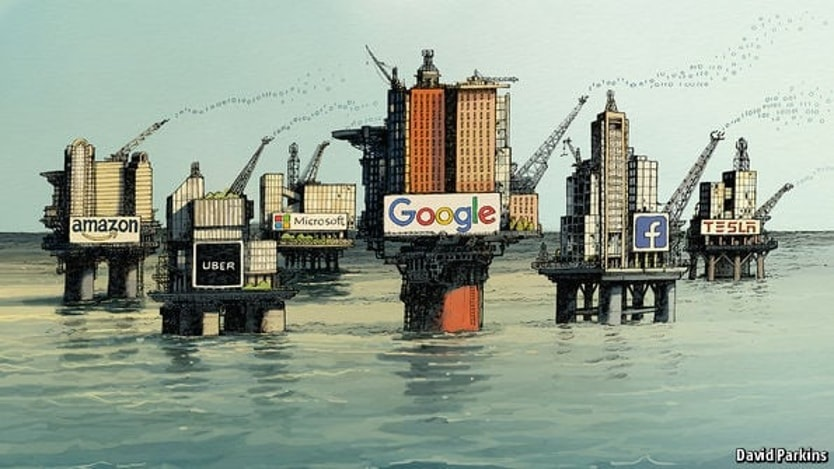
\includegraphics[scale=0.5]{figures/dados1.jpeg}
%    \caption{Caption}
%    \label{fig:my_label}
%\end{figure}


\newpage
\subsection{Histogramas}

\inic O histograma é um gráfico de barras no qual a escala horizontal representa classes de valores de dados e a escala vertical representa frequências. As alturas dos barras correspondem aos valores das frequências, e as barras são desenhadas adjascente uma às outras (sem separação).
 \vskip0.3cm
 
\inic O histograma é formado por um conjunto de retangulos justapostos
que tem as bases sobre um eixo horizontal, com centro no ponto
médio. As bases coincidem com as amplitudes de classe, e as
alturas devem ser proporcionais as frequências das
classes.
\vskip0.3cm 
 

\inic Os histogramas em geral apresentam a medição de interesse no eixo
x e o número ou percentagem de observações no eixo y, embora
alguns programas de computador façam o oposto. 
\vskip0.3cm

Se todos os intervalos tiverem a mesma amplitude, as alturas serão
proporcionais as frequências das classes, tornando-se então as
alturas numericamente iguais a essas frequências.\vskip0.3cm

ou seja,\vskip0.3cm

LARGURA DO RETÂNGULO = h(amplitude de classe)
ALTURA DO RETÂNGULO = f(frequência de classe)


%\vspace{-2cm}
\begin{figure}
    \centering
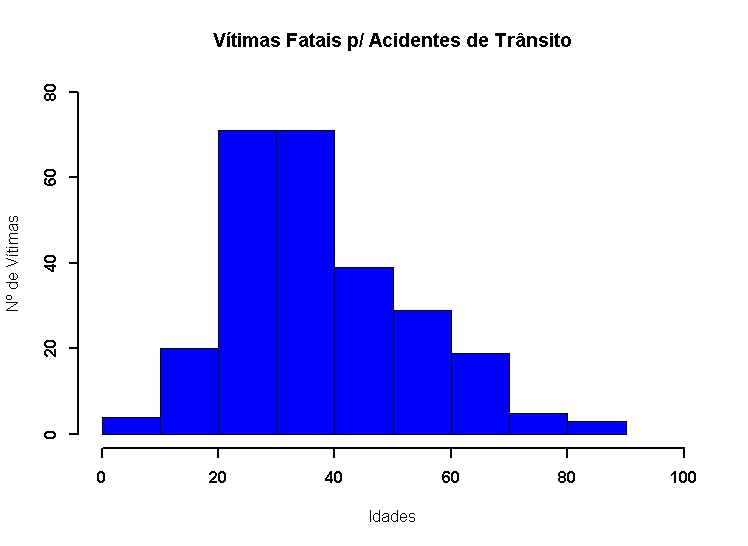
\includegraphics[scale=0.40]{figures/histograma1.jpeg}
    \caption{Histograma das Idades de Vítimas Fatais por Acidentes de Trânsito, Belém em 2022.}
    \label{fig:my_label25}
\end{figure}

%\vspace{-2cm}
\begin{figure}
    \centering
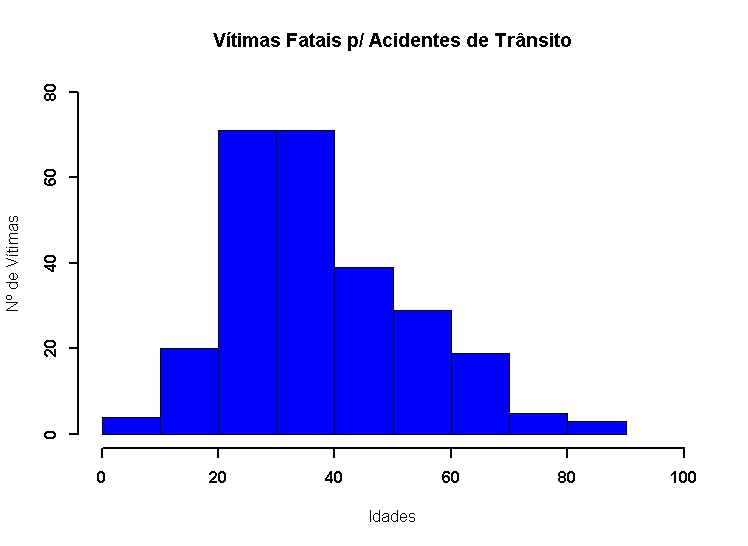
\includegraphics[scale=0.4]{figures/histograma1.jpeg}
    \caption{Histogram das Idades de Vítimas Fatais por Acidentes de Trânsito, Belém em 2022.}
    \label{fig:my_label23}
\end{figure}







\newpage
\subsection{Polígono de Frequência Simples e Acumulado}

È um gráfico de linhas, sendo as frequência marcadas sobre as
perpendiculares levantadas pelos pontos médios das classes. È a representação gráfica das frequências acumuladas. Usa-se
quando deseja saber qual parcela da população encontra-se até um
determinado valor, ou qual parcela encontra-se após um determinado
valor.\vskip0.3cm

O polígono de frequência é traçado marcando-se as frequências
acumuladas sobre os pontos correspondente aos limites superiores
dos intervalos de classe, também, conhecido como \textbf{Ogiva de
Galton}. A partir da Ogiva de Galton, pode-se fazer uma
interpolação linear, estimar valores de frequências acumuladas, de
uma distribuição em classes de frequências.\vskip0.3cm

A ogiva de galton, ou também chamada de \textbf{Gráfico de
Frequências Acumuladas}, concentra no limite superior de cada
classe a quantidade de elementos inferiores ou iguais a esse
limite superior. Dessa, forma, pode-se estimar a frequência
acumulada para um determinado valor que pertença a qualquer
intervalo que tiver sido usado para construir a ogiva. Para
determinadar esse valor, faz-se uma interpolação linear da ogiva.


\newpage

\vspace{-1cm}
\begin{figure}[H]
    \centering
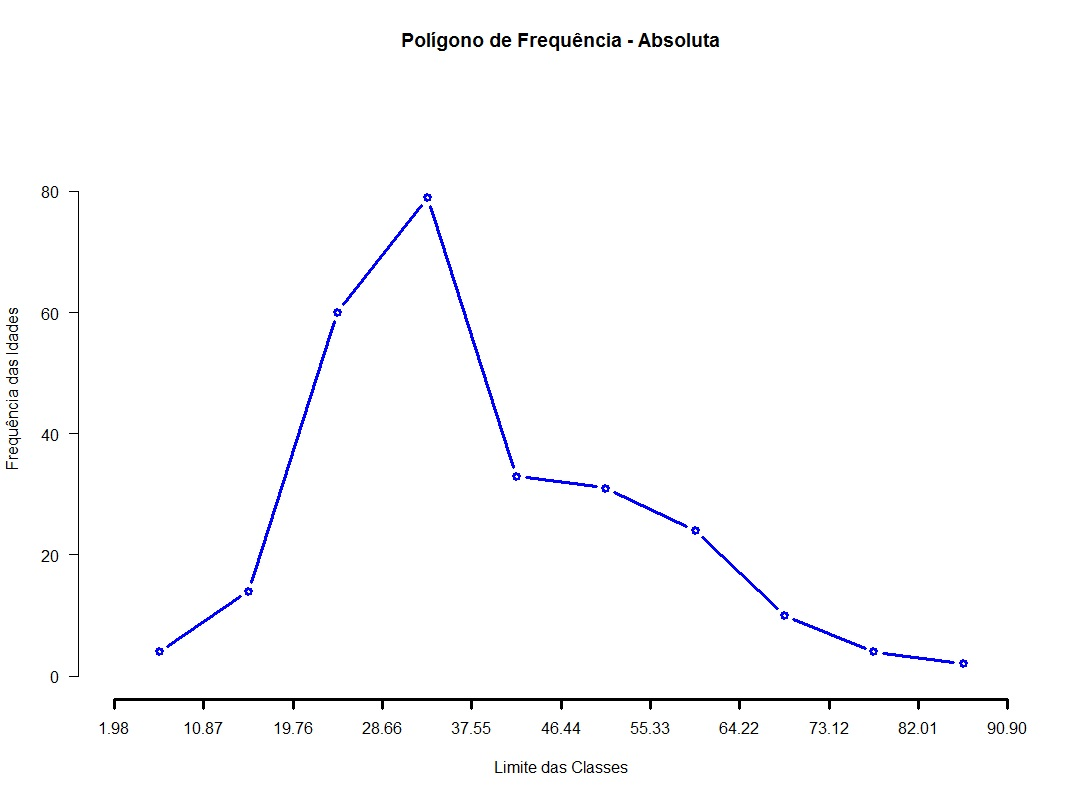
\includegraphics[scale=0.4,height=240pt,width=15cm]{figures/poligono1.jpeg}
    \caption{\textbf{Polígono de Frequências Absoluta} das Idades de Vítimas Fatais por Acidentes de Trânsito, Belém em 2022.}
    \label{fig:my_label25}
\end{figure}

\vspace{-2cm}
\begin{figure}
    \centering
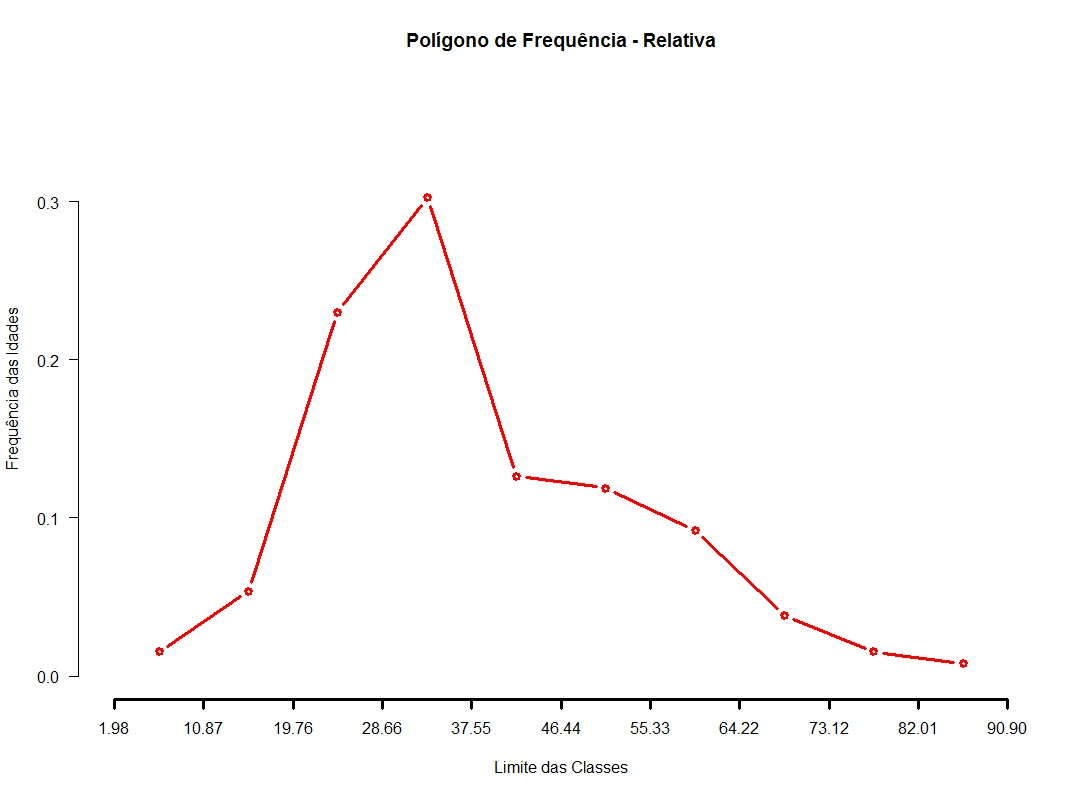
\includegraphics[scale=0.4,height=240pt,width=15cm]{figures/poligono2.jpeg}
    \caption{\textbf{Polígono de Frequências Relativa} das Idades de Vítimas Fatais por Acidentes de Trânsito, Belém em 2022.}
    \label{fig:my_label25}
\end{figure}


\newpage
\subsection{Gráfico de Barras (Simples ou Múltiplas)}

\inic O gráfico de barras é composto por duas linhas ou eixos, um
vertical e outro horizontal. No eixo vertical são construídas as
barras que representam a variação de um fenômeno ou de um processo
de acordo com sua intensidade. Essa intensidade é indicada pela
altura da barra. No eixo horizontal especifica-se as categorias da
variavel. As barras devem sempre possuir a mesma largura e a
distância entre elas deve ser constante.\vskip0.3cm

Os Gráficos de Barra são uma das formas mais populares de representar a informação, principalmente pela facilidade de execução e leitura. Sendo utilizado para apresentar um conjunto de dados e também para comparar vários conjuntos de dados. O formato em barras devem ser utilizados para representar variáveis discretas ou qualitativas, em termos absolutos ou relativos, para comparar categorias de variáveis quantitativas ou representar a evolução de uma característica ao longo do tempo.\vskip0.3cm

A representação de valores negativos é desaconselhada em gráficos de barras, dado que, convencionalmente, aos valores negativos está associada uma barra numa posição descendente. De fato, a associação visual entre esquerda e direita e valores negativos e positivos, respectivamente, pode não ser directa para um leitor menos experiente. Por essa razão, devem ser utilizados gráficos de colunas quando existem valores negativos.\vskip0.3cm

Nos gráficos de barras não é admissível a quebra de escala por deixar de ser possível efectuar comparações verticais entre categorias. Uma quebra de escala é enganadora, porque mostra visualmente a existência de grandes variações nos dados que de fato, não existem.\vskip0.3cm 

Na representação da informação, por vezes, é importante organizar as categorias por ordem crescente ou decrescente para melhor compreender certos fenómenos implícitos. É igualmente comum ordenar alfabeticamente (ou geograficamente) as designações das categorias, nomeadamente nos casos em que se representam países ou outro tipo de unidades administrativas, mas tal nem sempre é a melhor opção. Se o mesmo conjunto de categorias é apresentado em mais do que um gráfico, então a posição relativa de cada categoria deve manter-se, ou seja, as categorias devem aparecer na mesma ordem em todos os gráficos. Da mesma forma, o tamanho e a escala dos gráficos deve ser o mesmo, se o objectivo for a comparação entre eles. \vskip0.3cm  

Quando as categorias não são todas discriminadas, existindo, por exemplo, uma que reúne as restantes categorias sob a designação de ‘Outros’, é aconselhável não a incluir na ordenação e reservar-lhe o último lugar (WALLGREN, 1996; SCHMID, 1992). Caso se utilizem cores para diferenciar as categorias, a categoria ‘Outros’, por ser a menos importante, deve ter uma cor que não se destaque (ex: cinzento). \vskip0.3cm

\inic O primeiro passo na construção do gráfico é ter os dados armazenados em objetos apropriados. No caso do gráfico de barras é necessário que os dados estejam armazenados em um vetor ou matriz.




%\inic Pode-se criar também, o gráfico de barras de duas ou mais
%variáveis, um ao lado do outro, na mesma janela gráfica.
%\subsection{Gráfico de Colunas (Simples ou Multiplas)}



\subsection{Gráfico de Linhas, Curvas ou Segmentos}

Este tipo de gráfico representa a série histórica, exclusivamente,
indicado para mostrar tendências e evolução de uma variável
contínua por outra variável contínua. Requer, entretanto, que tal
série apresente um número significativo de informações (5 ou
mais), ou melhor, para 5 ou número menor de ocorrências, outro
gráfico deve ser construído, o gráfico de colunas.\vskip0.3cm

O primeiro gráfico data do séc. X ou XI, mas só no fim do séc. XVIII surgiu na literatura. William Playfair foi responsável pela publicação do primeiro gráfico de linhas baseado em dados económicos. A reintrodução do sistema de coordenadas cartesianas em 1637 por René Decartes, responsável pela relação estabelecida entre uma linha e uma equação, enquadrou e deu corpo a este formato de representação de dados.\vskip0.3cm

A leitura dos dados em gráficos de séries temporais obedece a duas lógicas preferenciais: avaliação da tendência, crescente ou decrescente, da série de dados, e responder a perguntas do tipo: Em que período se localizou o maior aumento ou a maior diminuição? Quais foram os pontos de inflexão ou de inversão pontual da tendência? A escala logarítmica possibilita a comparação de séries cujos valores apresentam dimensões muito diferentes (ainda que os valores da escala deixem de poder ser lidos de forma direta). Em certas circunstâncias, deve ser equacionada a substituição destes formatos pelos gráficos de barras e gráficos de área.

\newpage
\subsection{Gráfico Circular, Setorial ou Pizza}

O gráfico circular, setorial ou também chamado de Pizza, é
utilizado para comparar os valores de cada parcela de um conjunto
de dados com o total. É feito tomando por base a figura de um
círculo dividido em setores de tamanhos proporcionais aos valores
que representam. Os valores são expressos em números ou em percentuais. \vskip0.3cm

Algumas recomendações devem ser feitas para a elaboração dos
Setogramas. Os valores devem ser apresentados em ordem
decrescente a partir da parte superior do gráfico e no sentido
horário.\vskip0.3cm

A sua utilização é desaconselhada quando se pretende comparar mais
de um período temporal, para variáveis que contenham até cinco
categorias ou quando as categorias têm aproximadamente o mesmo
peso, sob pena de perder umas das principais funçoes: a da
comparação, sendo neste caso, preferível substituir o gráfico de
setores por um gráfico de barras.\vskip0.3cm

Quando a variável é do tipo \textbf{Ordinal}, gráficos de colunas são mais indicados pelo fato de permitirem manter a ordem das categorias (BARBETA, 2010).



%\begin{figure}[H]
%    \centering
%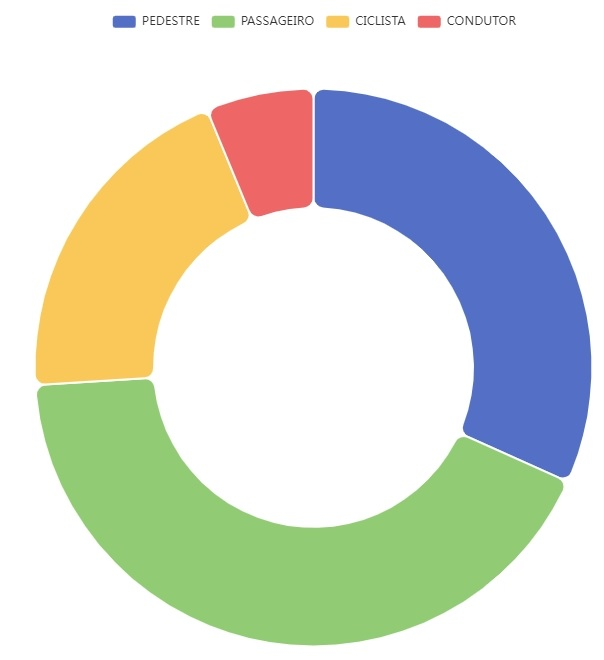
\includegraphics[scale=0.20,height=250pt,width=11cm]{figures/Rosca.jpeg}
%    \caption{Condição das Vítimas Não Fatal por Acidentes de Trânsito, Registrados no Município de Belém, Estado do Pará, no período de 2016 a 2022.}
%    \label{fig:my_label300}
%\end{figure}







%\newpage
%\subsection{Gráfico Polar}

%È a representação de uma série histórica ou temporal por meio de
%círculos concêntricos divididos em setores de iguais dimensões e
%em quantidades, de acordo com a variabilidade do fato estudado. A
%representação dos dados resultará na composição ou de um polígono
%ou do traçado de linhas radiais proporcionais aos valores que
%representam, as quais servirão de recursos visuais para a
%interpretação das informações. Muito utilizados para a
%representação de dados sobre abordagens de operações da Lei Seca
%pelos agentes de fiscalização de forma mensal.



\newpage
\subsection{Gráfico Radar ou Polar}

O gráfico radar é utilizado para representar fenômenos cuja
apresentação é feita em três ou mais variáveis quantitativas em eixos que partem do mesmo ponto. A sua análise exige mais
atenção em virtude da maior complexidade da sua apresentação. 



\begin{figure}[H]
    \centering
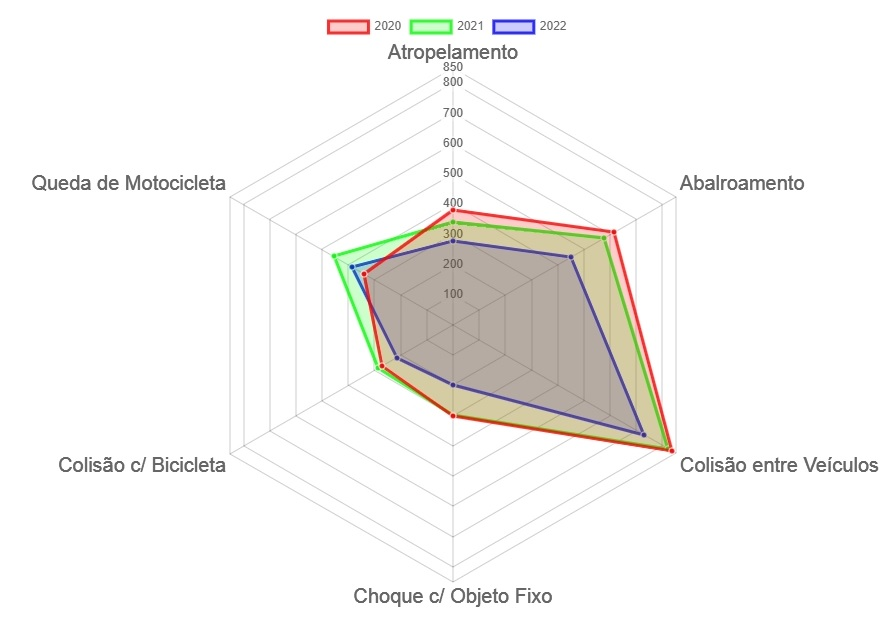
\includegraphics[scale=0.25,height=260pt,width=12cm]{figures/radarplot1.jpeg}
    \caption{Acidentes de Trânsito por Tipo, Registrados no Município de Belém, Estado do Pará, no período de 2020 a 2022.}
    \label{fig:my_label30}
\end{figure}


O gráfico de radar é também conhecido como gráfico de \textbf{Teia}, \textbf{Aranha}, \textbf{Estrela}, \textbf{Polígono Irregular}, \textbf{Polar}, ou \textbf{Diagrama Kivia} (Mosley e Mayer, 1999).


\newpage
\subsection{Gráfico em Pirâmide Etária}

A pirâmide etária é também um histograma e é muito utilizada em  análises demográficas por permitir visualizar numa única imagem a distribuição da população por idades e silutaneamente compará-las entre os gêneros. A representação em valores absolutos fornece a dimensão dos dados mas impede qualquer tipo de comparação no espaço ou no tempo, que apenas é possível se os dados foram apresentados em termos relativos (NAZARETH, 1996). 
\vskip0.3cm

A pirâmide etária é uma forma de representar a estrutura da
população por idade e gênero. O eixo horizontal representa o
número absoluto ou relativo da população e o eixo vertical
representa os grupos etários e são normalmente apresentados em grupos etários em cinco anos, mas também podem ser representados ano a ano. O lado direito do eixo horizontal é destinado à representação do contingente ou proporção de mulheres e o esquerdo, dos homens.



\begin{figure}[H]
    \centering
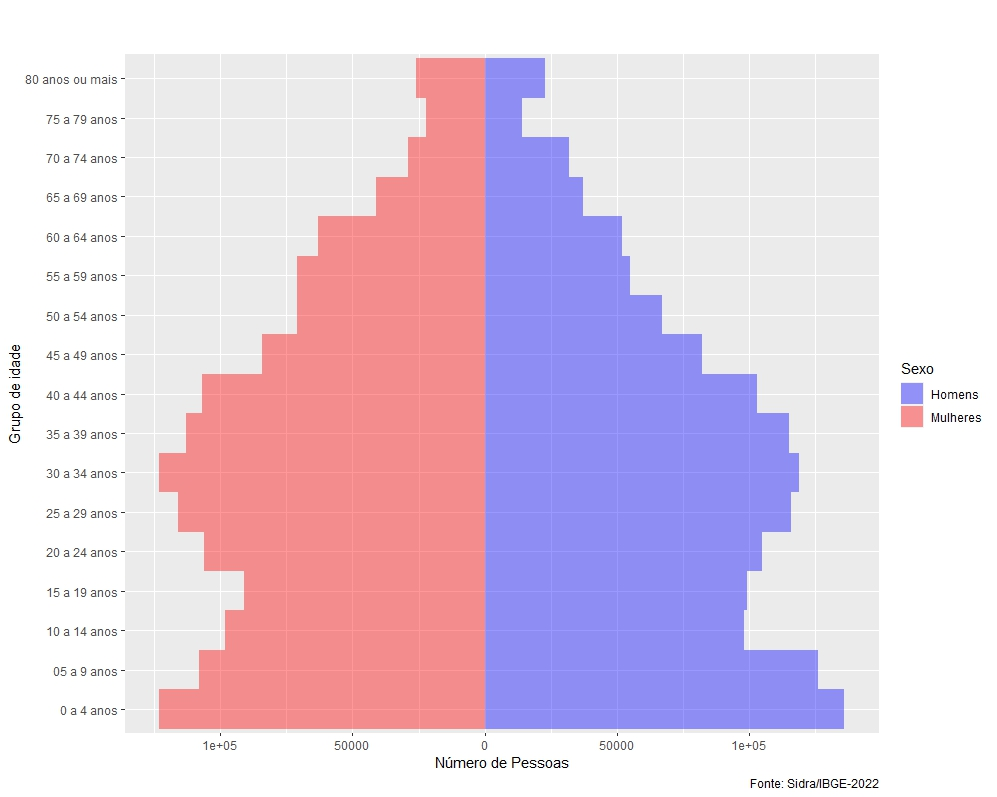
\includegraphics[scale=0.25,height=260pt,width=12cm]{figures/piramide1.jpeg}
    \caption{Pirâmide Etária da População Residente, segundo Faixa Etária no Município de Belém, Estado do Pará - 2022.}
    \label{fig:my_label30}
\end{figure}

















\newpage
\subsection{Gráfico em Cartograma}

O cartograma é a representação sobre uma carta geográfica (mapa).
Também chamado de Esteriográfico é empregado quando o objetivo é o de
figurar os dados estatísticos diretamente relacionados com áreas
geográficas ou políticas.



\begin{figure}[H]
    \centering
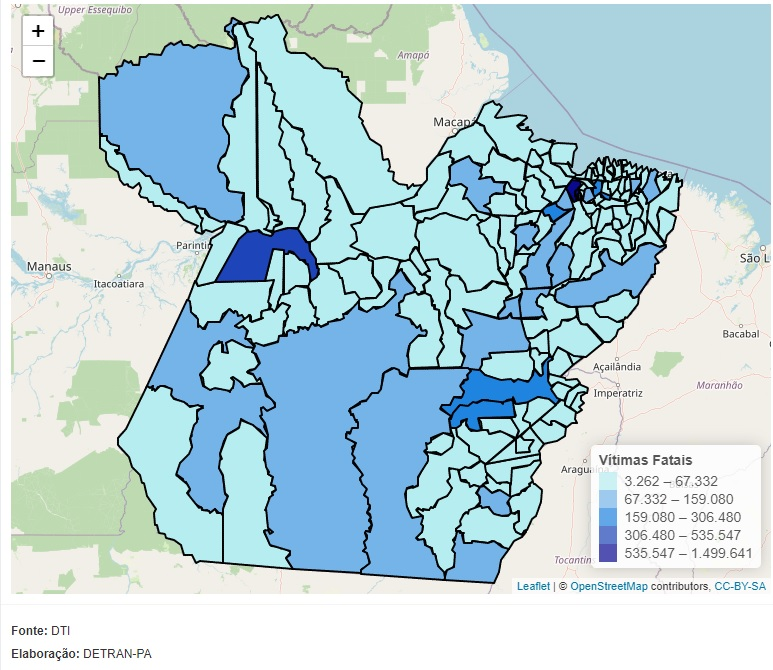
\includegraphics[scale=0.25,height=270pt,width=12cm]{figures/Map1.jpeg}
    \caption{Vítimas Fatais por Acidentes de Trânsito, Municípios do Estado do Pará em 2022.}
    \label{fig:my_label25}
\end{figure}


Os cartogramas representam as quantidades que correspondem a cada divisão, o uso de cores e suas tonalidades dispostas segundo uma intensidade visual crescente de modo que os valores absolutos ou relativos sejam representados a partir do menor para o maior de maneira coerente e proporcional. 


%\vspace{-16cm}
%\begin{figure}[H]
%    \centering
%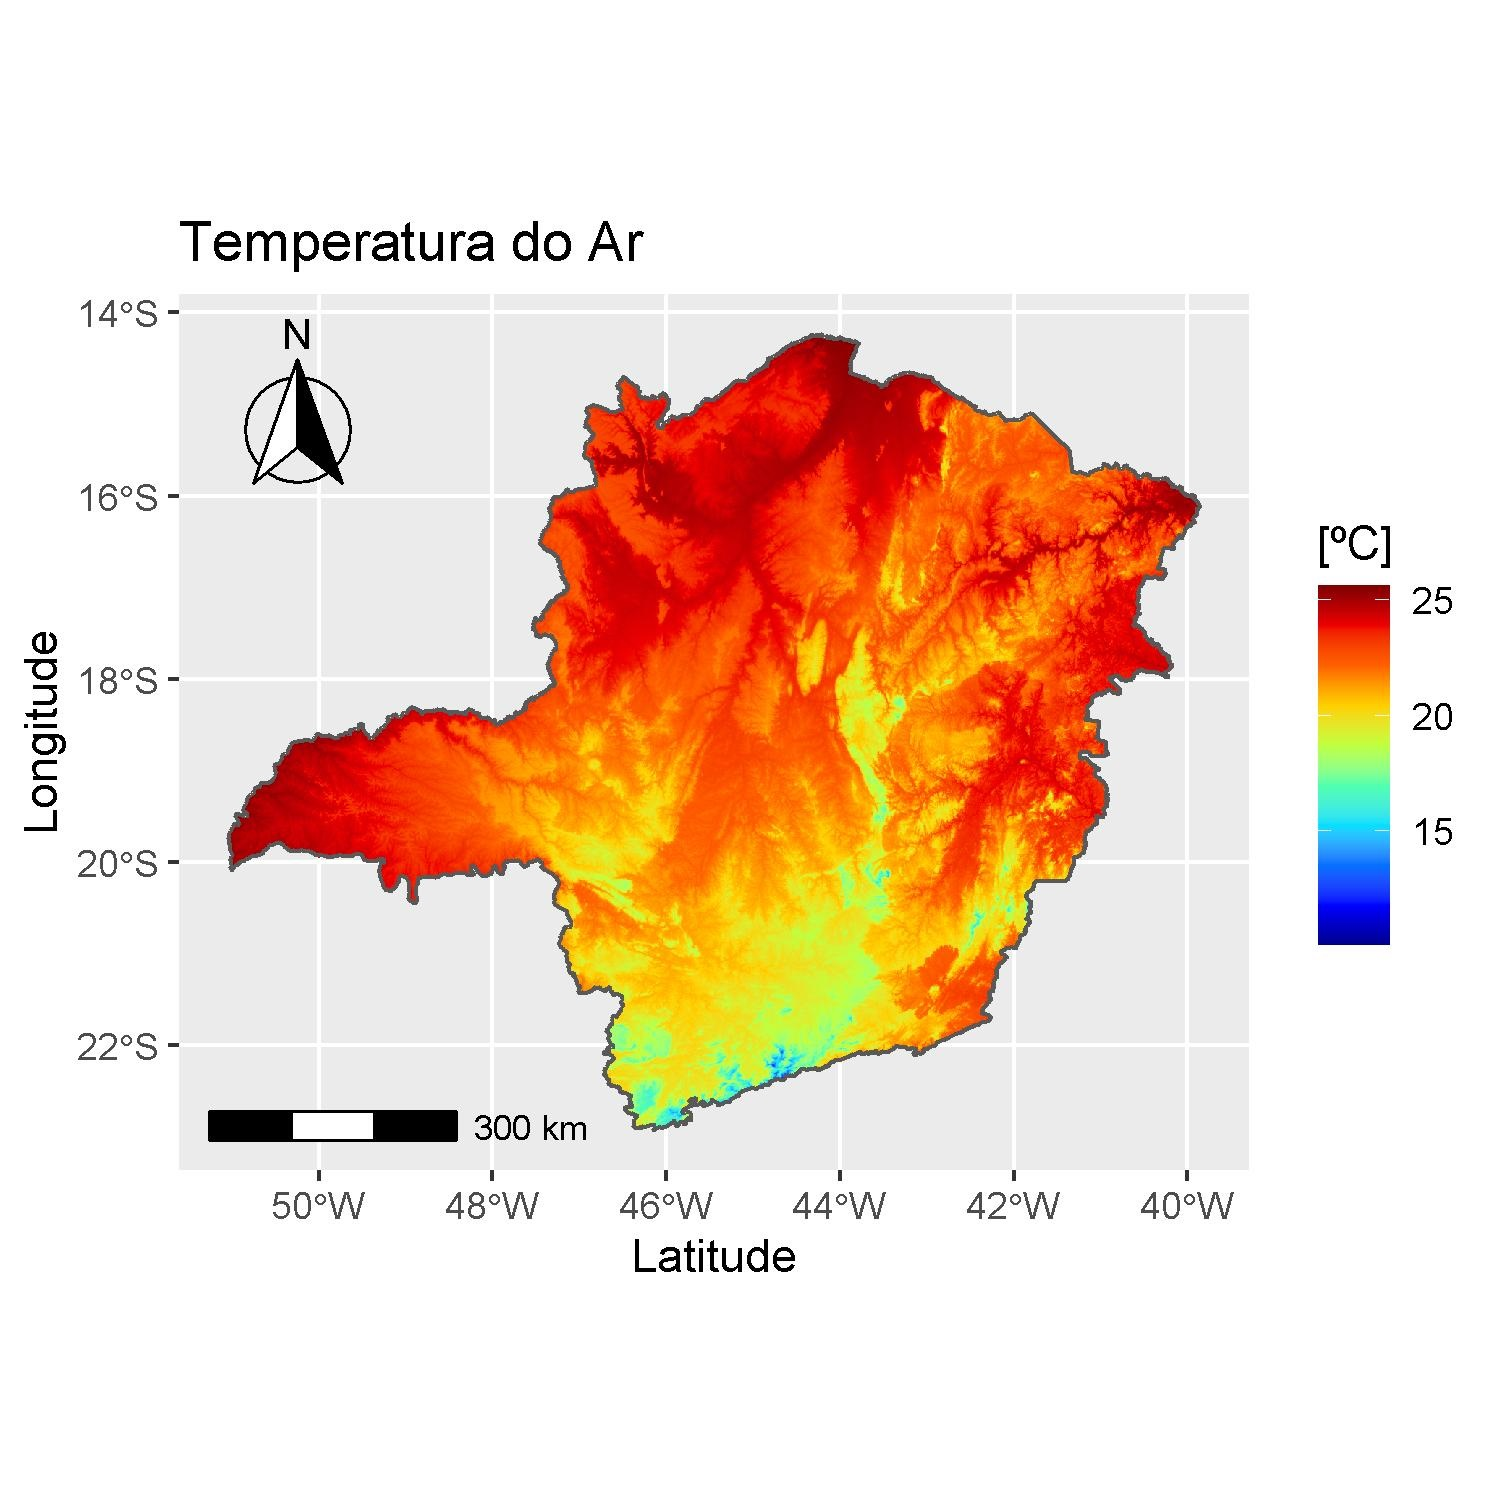
\includegraphics[scale=0.85,height=600pt,width=25cm]{figures/Temperatura1.jpeg}
%    \caption{Temperatura do Ar em Minhas Gerais de janeiro a dezembro de 2022.}
%    \label{fig:my_labelmap1}
%\end{figure}




\newpage
\subsection{Gráfico Ilustrativo, Diagrama Símbólico, Pictórico ou Pictograma}

O pictograma constitui um dos processos gráficos que melhor fala
ao público, pela sua forma ao mesmo tempo atraente e sugestiva. O
pictograma é um gráfico representado através de figuras que
simbolizam fatos estatísticos, ao mesmo tempo que indicam
proporcionalidade. São gráficos que carecem de precisão, mas, como
são muitos atrativos, são largamente usados em revistas voltadas
ao público em geral e publicidades na segurança pública. Não é
utilizado em trabalhos científicos.\vskip0.3cm

Os diagramas simbólicos são frequentemente usados para apresentar os dados estatísticos de modo a despertar a atenção do público em geral, e apresentando grande dose de originalidade e de habilidade na arte de apresentação dos dados.\vskip0.3cm

Os pictogramas mais usuais são os baseados no critério do tamanho: em que a variação em área do tamanho das formas utilizadas é proporcional à variação da variável representada.\vskip0.3cm



\textbf{Regras Fundamentais para a Construção de um Pictograma}

\begin{enumerate}
    \item Os símbolos devem explicar-se por si próprios.
    \item As quantidades maiores são indicadas por meio de um
    número maior de símbolos, mas não por um símbolo maior.
    \item Os símbolos comparam quantidades aproximadas, não
    detalhes minuciosos.
    \item Os gráficos pictóricos só devem ser usados para
    comparações, nunca para afirmações detalhadas ou isoladas.
\end{enumerate}






\begin{figure}[H]
    \centering
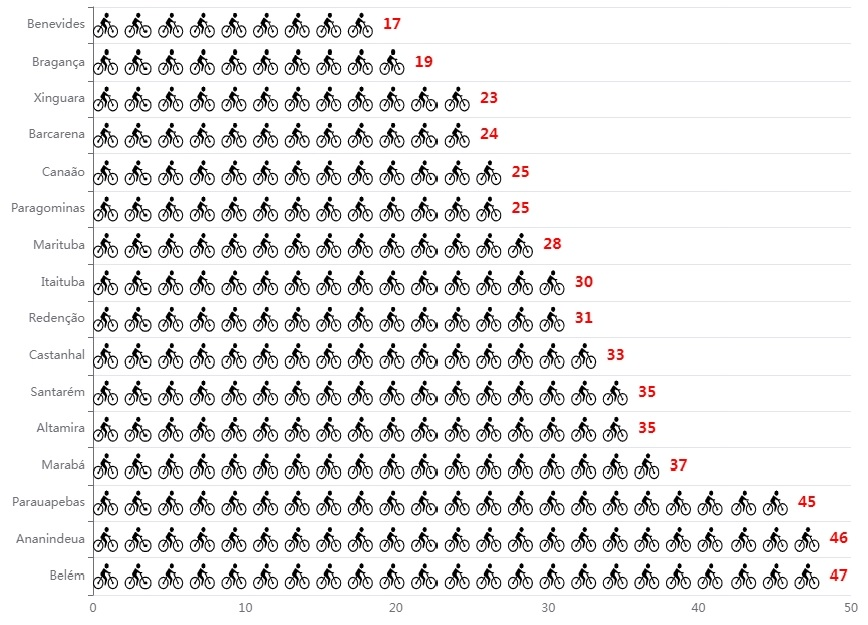
\includegraphics[scale=0.25,height=230pt,width=12cm]{figures/pictograma1.jpeg}
\vspace{-0.5cm}
    \caption{Pictograma de Vítimas Fatais por Acidentes de Trânsito com Bicicleta, em alguns Municípios do Estado do Pará - 2022.}
    \label{fig:my_label50}
\end{figure}

\vspace{-0.85cm}
\begin{figure}[H]
    \centering
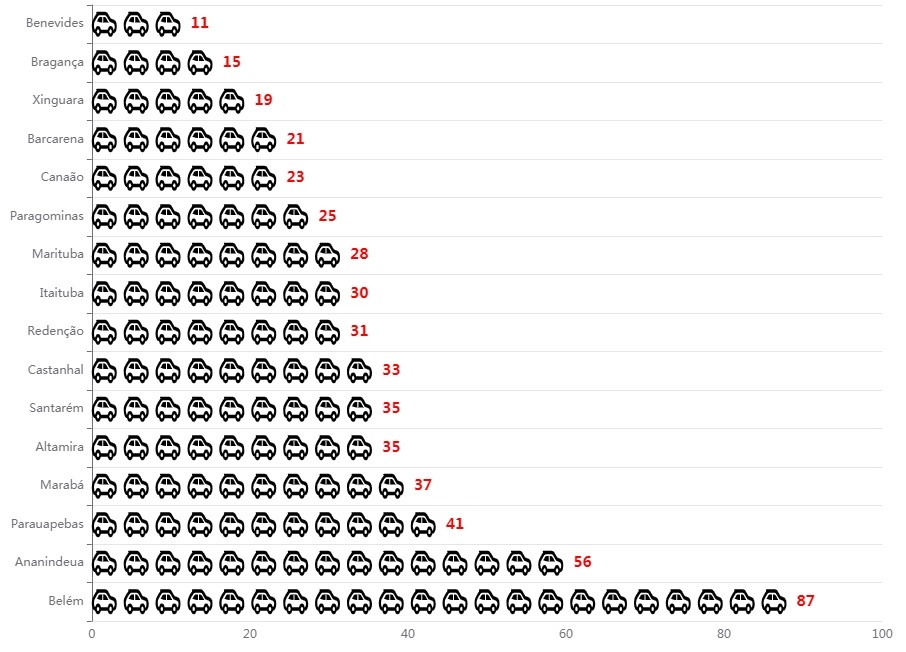
\includegraphics[scale=0.25,height=230pt,width=12cm]{figures/pictograma2.jpeg}
\vspace{-0.5cm}
    \caption{Pictograma de Vítimas Fatais por Acidentes de Trânsito com Automóvel em alguns Municípios do Estado do Pará - 2022.}
    \label{fig:my_label51}
\end{figure}






















\newpage 
\subsection{Diagrama de Caixa, Bigodes, Whisker ou Box Plot}

\inic Em 1977, o estatístico John Wilder Tukey propôs um dispositivo visual útil
para a comunicação de características de uma série de dados que se
tornou bastante famoso. Conhecido enormemente no meio acadêmico
como Box-Plot, na qual é um tipo de gráfico que objetiva
apresentar diversas informações sobre o comportamento dos dados e
ainda manter uma forma compacta. 

\vspace{-1.5cm}
\begin{figure}
    \centering
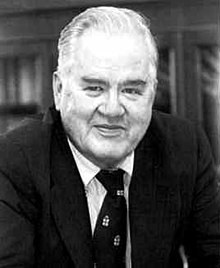
\includegraphics[scale=0.6]{figures/John_Tukey.jpeg}
    \caption{John Wilder Tukey (1915-2000)}
    \label{fig:my_label25}
\end{figure}



Na análise das informações, pode
ser importante a construção de um diagrama em caixa, contendo as
seguintes informações: valores mínimos e máximos, a mediana, o
primeiro e o terceiro quartil, na qual representa 25\% e 75\% da
distribuição de freqüência.\vskip0.3cm




\begin{figure}[!htb]
\centering{
 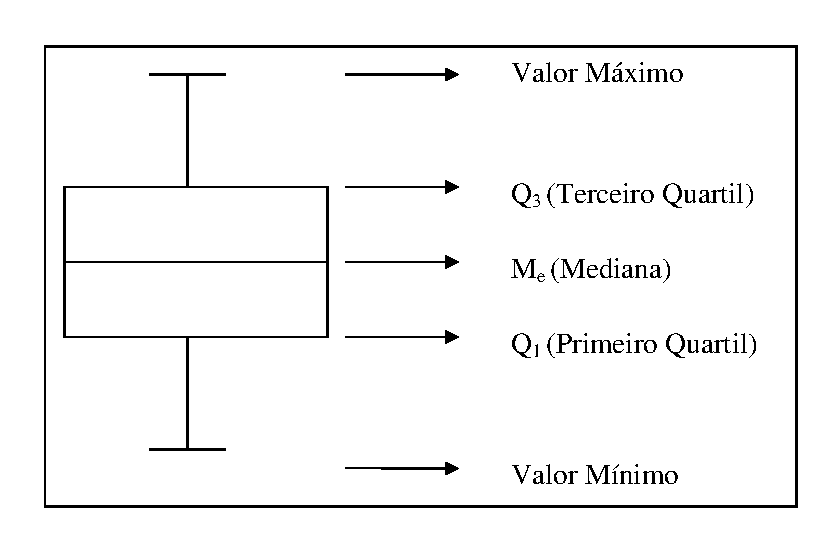
\includegraphics[scale=0.65]{figures/Boxcaixa.eps}\\
  \vspace{-0.2cm}
  \caption{Esquema Geral sobre o diagrama de caixas ou Box Plot.}\label{esquematabela}
  }
\end{figure}


\newpage
\inic As linhas verticais que saem do diagrama foram chamadas whiskers
por Tukey, essas linhas servem de elo entre os valores mais
centrais e os extremos da série de dados, geralmente representam
os valores mínimos e máximos.\vskip0.3cm 


A mediana da série é representada
por uma linha horizontal central no diagrama, e o quartil inferior
(Q1) e superior (Q3), pelas linhas inferior e superior que
delimitam a caixa.\vskip0.3cm  

A mediana representa uma estimativa de tendência central, e a altura da do diagrama, uma estimativa da variabilidade geral dos
dados. Na qual a posição da mediana, seja ela central ou mais
próxima a um dos quartis, indica a presença ou não de assimetria
nos dados.\vskip0.3cm


\inic Ao explorar um conjunto de dados de forma gráfica, deve-se considerar os valores discrepantes ou Outliers, pois eles podem revelar importantes informações e podem afetar grandemente os valores da média e do desvio-padrão, bem como disfarçar seriamente um histograma, ou seja,, um outlier pode ter efeito um dramático sobre a escala do gráfico, de modo que a verdadeira natureza da distribuição pode ser totalmente  obscurecida.



\newpage

\vspace{-3cm}
\begin{figure}[H]
    \centering
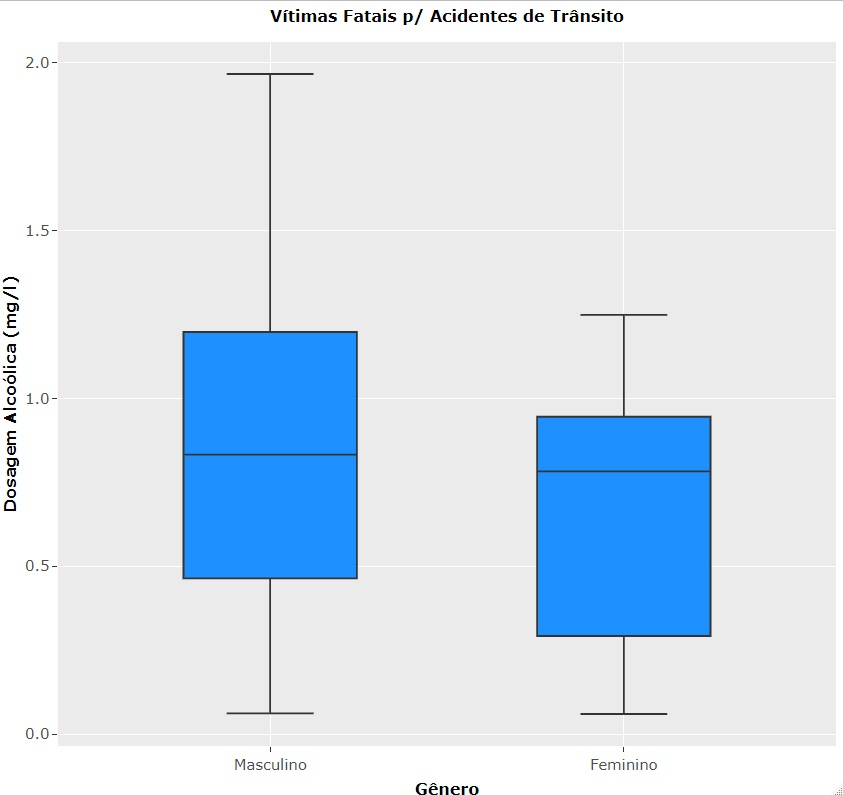
\includegraphics[scale=0.26,height=242pt,width=12cm]{figures/boxplot_dosagem.jpeg}
    \caption{\textbf{BoxPlot Tradicional}: Dosagem Alcoólica de Vítimas Fatais por Acidentes de Trânsito, Região Metropolitrana de Belém em 2022.}
    \label{fig:my_label25}
\end{figure}



\vspace{-2cm}
\begin{figure}[H]
    \centering
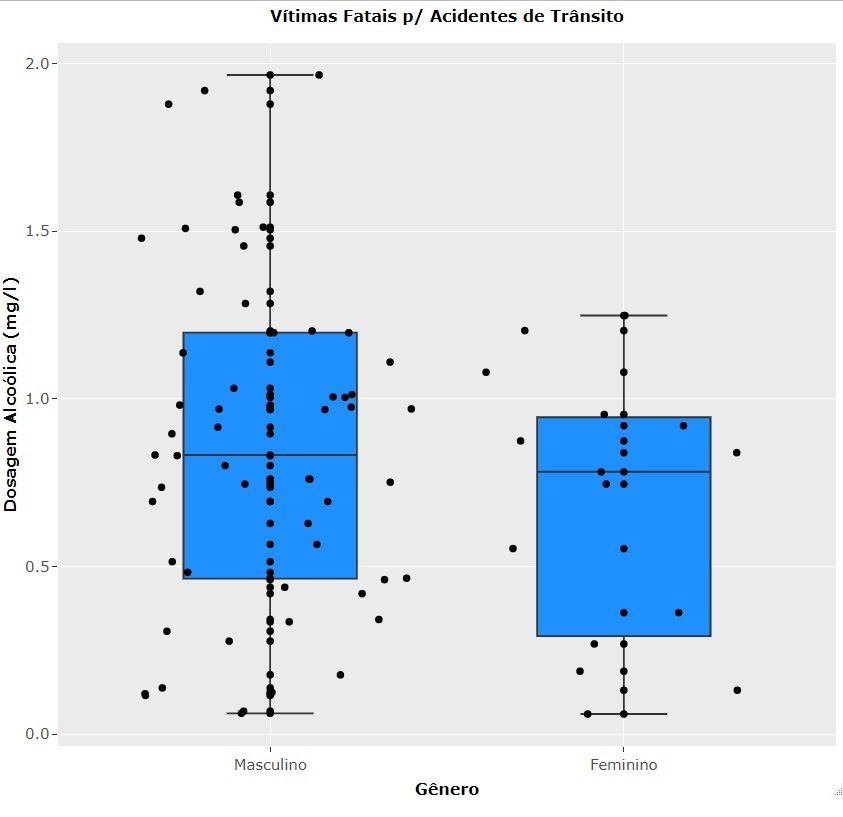
\includegraphics[scale=0.26,height=242pt,width=12cm]{figures/boxplot_dosagem_jitter.jpeg}
    \caption{\textbf{BoxPlot com Efeito Jitter}: Dosagem Alcoólica de Vítimas Fatais por Acidentes de Trânsito, Região Metropolitrana de Belém em 2022.}
    \label{fig:my_label25}
\end{figure}







\subsection{Gráfico de Violino, ViolinPlot}

O gráfico chamado de Violino, é muito utilizado quando se quer unificar a visualização do histograma junto com a do Boxplot, ou seja um casamento entre histogramas e boxplots. Observe que quanto menor o desvio padrão, mais concentrado são os dados, sendo refletido tanto no histograma como no boxplot. A vantagem do uso do \textbf{ViolinPlot} é que, além  das informações que o boxplot traz consigo, traz a densidade dos dados. 



\vspace{-2cm}
\begin{figure}[H]
    \centering
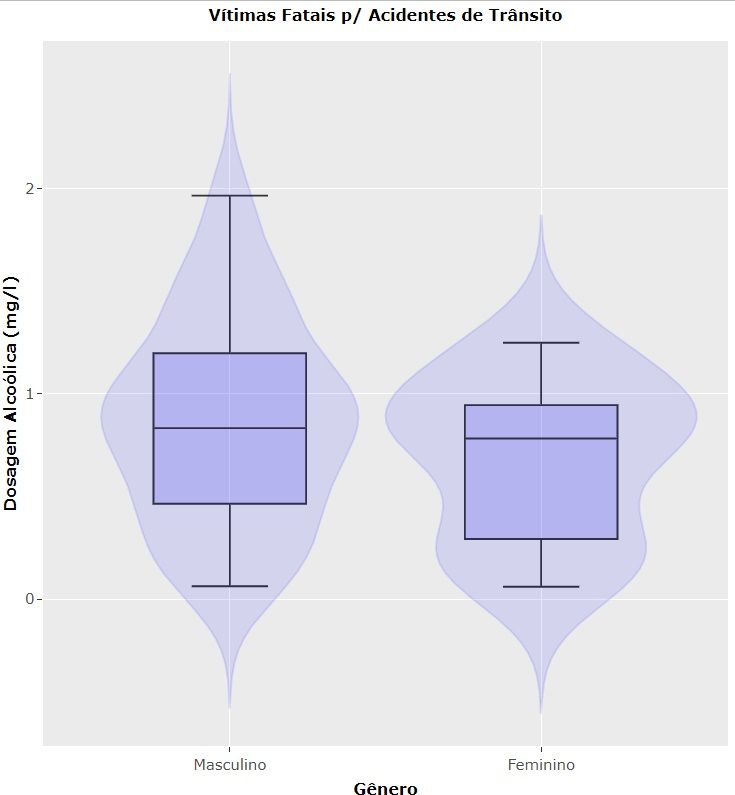
\includegraphics[scale=0.21,height=200pt,width=11cm]{figures/violinplot_Tradicional.jpeg}
    \caption{\textbf{ViolinoPlot com BoxPlot Tradicional}: Dosagem Alcoólica de Vítimas Fatais por Acidentes de Trânsito, Região Metropolitrana de Belém em 2022.}
    \label{fig:my_label25}
\end{figure}



\vspace{-2cm}
\begin{figure}[H]
    \centering
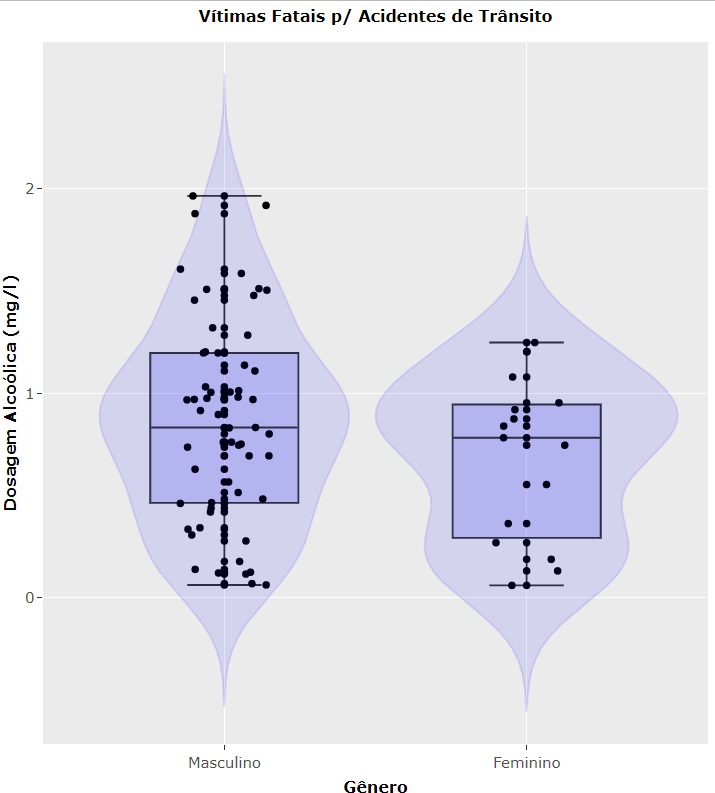
\includegraphics[scale=0.21,height=200pt,width=11cm]{figures/violinplot_jitter.jpeg}
    \caption{\textbf{ViolinoPlot com BoxPlot e Efeito Jitter}: Dosagem Alcoólica de Vítimas Fatais por Acidentes de Trânsito, Região Metropolitrana de Belém em 2022.}
    \label{fig:my_label25}
\end{figure}









%\newpage
%\subsection{Resumo Geral Sobre os Principais Gráficos}

%\inic Atualmente existem diversos tipos de gráficos, onde a escolha %depende do tipo de dado coletado e da informação que se pretende %transmitir. Cada um possui um conjunto de vantagens e desvantagens.      

%\begin{quadro}[h!tp]
%    \centering
%    \caption{Resumo geral sobre os principais gráficos mostrando suas %descrição, vantagens e desvantagens}
%    \begin{tabular}{|c|c|c|c|}
%   \hline\hline
%    Gráficos       & Descrição &  Vantagens          & Desvantagens %\\   
%\hline\hline
%  Barras           &           &  Fácil de Construir &             \\
%  \hline
%  Barras Agrupadas &           &                     &              \\
%  \hline
%  Linhas           &           &                     &              %\\  
%  \hline
%  Setores          &           & Analisar Proporção  &              \\
%  \hline
% Histograma       &           &  Mostra a distribuição         &      %        \\
%  \hline
%  Polígono         &           &           &              \\
%  \hline
%  Box Plot         &           &           &              \\
%\hline\hline
%\end{tabular}
%\end{quadro}









